% File: solutions/ex7.tex
\begin{soluzione}{7}
    L'obiettivo è determinare la forma dello spettro $X_R(f)$ dopo che lo spettro campionato con aliasing, $\tilde{X}(f)$, è stato processato da un filtro passa-basso ideale.
    \subsubsection*{1. Definizione dello Spettro Ricostruito}
    Lo spettro ricostruito è dato dal prodotto:
    \[
        X_R(f) = \tilde{X}(f) \cdot H_R(f)
    \]
    Dal testo del problema e dall'esercizio precedente, abbiamo:
    \begin{itemize}
        \item $\tilde{X}(f) = \sum_{k=-\infty}^{\infty} 150 \cdot X(f - k \cdot 150)$, dove $X(f)$ è lo spettro triangolare.
        \item $H_R(f)$ è un filtro passa-basso ideale con banda passante da $-75$ Hz a $75$ Hz e guadagno unitario. Matematicamente:
        \[
             H_R(f) = \text{rect}\left(\frac{f}{150}\right)
        \]
    \end{itemize}
    Questo significa che $X_R(f)$ sarà uguale a $\tilde{X}(f)$ per $|f| \le 75$ Hz, e zero altrove. Dobbiamo quindi calcolare la forma di $\tilde{X}(f)$ in questo intervallo.

    \subsubsection*{2. Analisi delle Componenti Sovrapposte}
    {\sloppy
    Nella banda $|f| \le 75$ Hz, contribuiscono due repliche spettrali:
    \begin{enumerate}
        \item \textbf{La replica centrale (k=0):} Contribuisce con l'espressione $150 \cdot X(f) = 150 \left(1 - \frac{|f|}{100}\right)$.
        \item \textbf{Le repliche adiacenti (k=$\pm$1):} 
            \begin{itemize}
                \item Per $f > 0$, la replica di sinistra (centrata a -150 Hz) non contribuisce, ma quella di destra (centrata a 150 Hz) contribuisce nell'intervallo $[50, 75]$ Hz. La sua espressione è $150 \cdot X(f-150) = 150 \left(1 - \frac{|f-150|}{100}\right)$.
                \item Per $f < 0$, la replica di destra non contribuisce, ma quella di sinistra (centrata a -150 Hz) contribuisce nell'intervallo $[-75, -50]$ Hz. La sua espressione è $150 \cdot X(f+150) = 150 \left(1 - \frac{|f+150|}{100}\right)$.
            \end{itemize}
    \end{enumerate}
    }
    
    \subsubsection*{3. Calcolo dell'Espressione Analitica}
    Dividiamo il calcolo in due regioni, data la simmetria.
    \textbf{Regione A: $0 \le f < 50$ Hz}
    In questa regione, solo la replica centrale contribuisce.
    \[
        X_R(f) = 150 \left(1 - \frac{f}{100}\right)
    \]
    
    \textbf{Regione B: $50 \le f \le 75$ Hz}
    In questa regione, sia la replica centrale sia quella di destra (centrata a 150 Hz) si sommano.
    \begin{itemize}
        \item Contributo centrale: $150 \left(1 - \frac{f}{100}\right)$
        \item Contributo della replica destra: $150 \left(1 - \frac{|f-150|}{100}\right) = 150 \left(1 - \frac{150-f}{100}\right)$ poiché $f < 150$.
    \end{itemize}
    Sommando i due contributi:
    \begin{align*}
        X_R(f) &= 150 \left(1 - \frac{f}{100}\right) + 150 \left(1 - \frac{150-f}{100}\right) \\
        &= 150 \left[ \left(1 - \frac{f}{100}\right) + \left(1 - 1.5 + \frac{f}{100}\right) \right] \\
        &= 150 \left[ 1 - \frac{f}{100} + 1 - 1.5 + \frac{f}{100} \right] \\
        &= 150 \left[ 2 - 1.5 \right] = 150 \cdot 0.5 = 75
    \end{align*}
    
    Lo spettro in questa regione è costante e vale 75.

    Mettendo insieme i pezzi, l'espressione completa per $X_R(f)$ è:
    \[ \mathbf{X_R(f) = 
        \begin{cases} 
            150 \left(1 - \frac{|f|}{100}\right) & \text{per } |f| < 50 \text{ Hz} \\
            75 & \text{per } 50 \le |f| \le 75 \text{ Hz} \\
            0 & \text{altrimenti}
        \end{cases}}
    \]

    \subsubsection*{4. Grafico dello Spettro Ricostruito}
    Il grafico risultante ha una punta triangolare al centro e delle "spalle" piatte dove è avvenuto l'aliasing.
    \begin{center}
    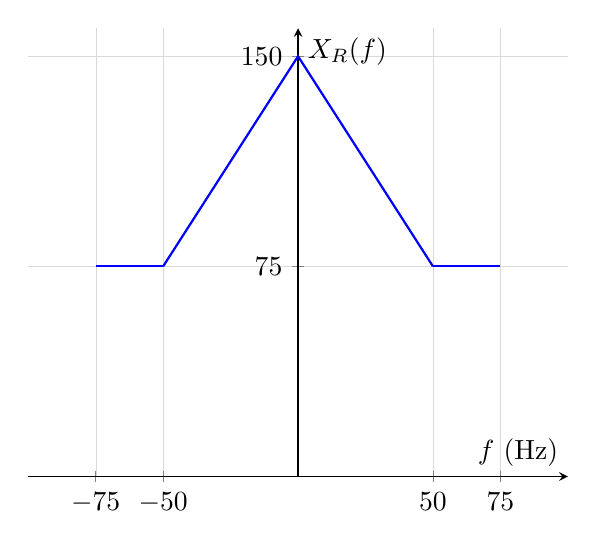
\begin{tikzpicture}
        \begin{axis}[
            axis lines=middle,
            xlabel=$f$ (Hz),
            ylabel=$X_R(f)$,
            xmin=-100, xmax=100,
            ymin=0, ymax=160,
            xtick={-75, -50, 0, 50, 75},
            ytick={75, 150},
            grid=both,
            grid style={line width=.1pt, draw=gray!30}
        ]
        % Parte centrale (triangolo)
        \addplot[blue, thick] coordinates { (-50, 75) (0, 150) (50, 75) };
        % Spalla destra (aliasing)
        \addplot[blue, thick] coordinates { (50, 75) (75, 75) };
        % Spalla sinistra (aliasing)
        \addplot[blue, thick] coordinates { (-75, 75) (-50, 75) };
        \end{axis}
    \end{tikzpicture}
    \end{center}
    
\end{soluzione}